\subsection*{Измерения}

Далее используются обозначения: $U_2$ -- задерживающий потенциал, $U_1$ -- ускоряющее напряжение, $I$ -- ток коллектора. 

\textbf{Динамический режим}. В динамическом режиме,  измерим ВАХ лампы $I(U)$, см. рис. \ref{fig:lamp}. Оцифруем полученные зависимости, и измерим для них $\Delta U$, см. таблицу \ref{tab:1}. 
\begin{figure}[h]
    \centering
    \includegraphics[width=0.6\textwidth]{figures/dynamic_v1.pdf}
    \caption{Измерение $\Delta U_1$ в динамическом режиме}
    \label{fig:lamp}
\end{figure}

Среднее значение для $\Delta U_{1, \text{dyn}}$ получилось: $ \Delta U_{1, \text{dyn}} = (18 \pm 1) \text{ В}.$ 
Погрешность обусловлена разбросом снятых с ВАХ значений. 


\textbf{Статический режим}. В статическом режиме, посмотрим на ВАХ лампы $I(U)$, см. таблицу 2. Погрешность измерений: $\sigma[U_1] = 0.1$ В, $\sigma[I] = 0.5\ \mu$А. Построим зависимость $I(U)$ для различных запирающих напряжений, см. рис. \ref{fig:1}.
\vspace{-12mm}
\begin{figure}[h]
    \centering
    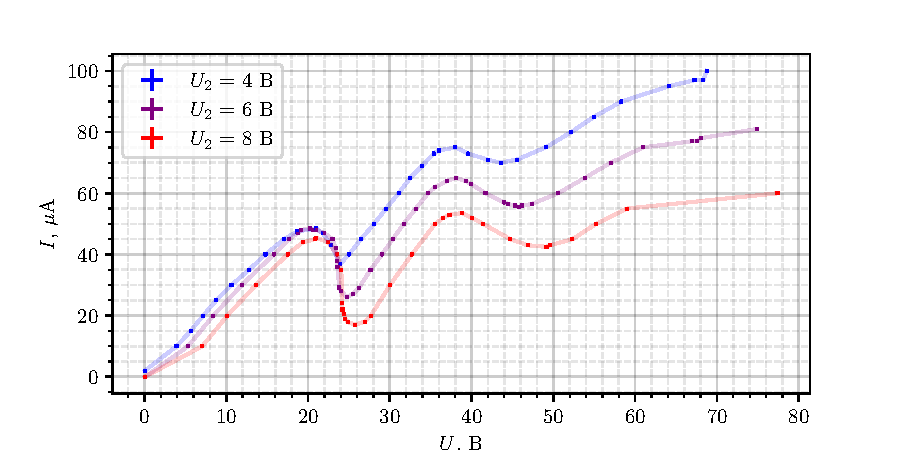
\includegraphics[width=0.92\textwidth]{figures/plot1.pdf}
    \caption{Измерение ВАХ в статическом режим при различных запирающих напряжения.}
    \label{fig:1}
\end{figure}

Определим максимумы и минимумы найденных зависимостей, см. таблицу 1. Заметим, что расстояние для максимумов и минимумов $\Delta U$ различается. Возможно, это связана с особенностями измерения максимумов и минимумов. Скорее всего это связано с особенностями установки.




\begin{table}[h]
    \centering
    \caption{Результаты измерения экстремумов}
    \begin{tabular}{c||cc|c||cc|c||c}
    \toprule
     $U_2$, В &  
     $U_1^{\text{min}_\text{I}}$, В &  
     $U_1^{\text{min}_\text{II}}$, В &  
     $\Delta U_1^{\text{min}}$, В &  
     $U_1^{\text{max}_\text{I}}$, В &  
     $U_1^{\text{max}_\text{II}}$, В  & 
     $\Delta U_1^{\text{max}}$, В &
     $\Delta U_{1, \text{dyn}}^{\text{min}}$, В 
     \\
    \midrule
      4 &  24.0 &  43.6 &   20 & 21.0 &  38.0 &       17 & 17 \\
      6 &  24.7 &  45.8 &   21 & 20.2 &  38.1 &       18 & 18 \\
      8 &  25.7 &  49.2 &   23 & 21.0 &  38.1 &       17 & 18 \\
    \bottomrule
    \end{tabular}
    \label{tab:1}
\end{table}

\newpage

\textbf{Про измерение максимумов}. 
В статическом режиме тщательно измерялись области вблизи экстремумов. За экстремум бралась точка такая, что изменения $U_1$ приводили к отступлению вверх/вниз от экстремума на $\sigma[I] = 0.5\ \mu$А. 

\begin{figure}[ht]
    \centering
    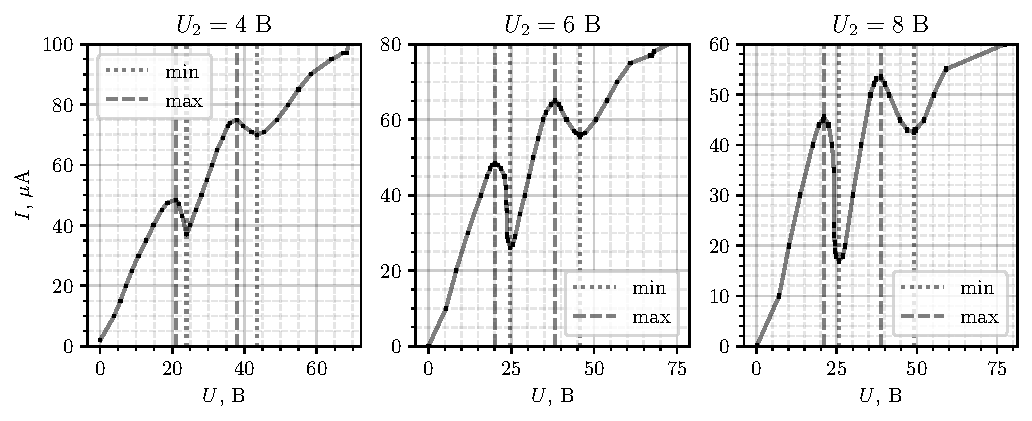
\includegraphics[width=\textwidth]{figures/plot2.pdf}
    \caption{Определение экстремумов ВАХ лампы в статическом режиме}
    \label{fig:2}
\end{figure}

На рис.  \ref{fig:2} приведены измеренные таким образом значения для экстремумов.



\textbf{Результат измерений}. Итого, средние значения для $\Delta U$ в статическом режиме получились:
\begin{align*}
    \Delta U_{1, \text{stat}}^{\text{min}} &= (21 \pm 1) \text{ В}, \\
    \Delta U_{1, \text{stat}}^{\text{max}} &= (17 \pm 1) \text{ В}, \\
    \Delta U_{1, \text{dyn}} &= (18 \pm 1) \text{ В}, \\
    \Delta U_{1, \text{table}} &= 21.6 \text{ В},
\end{align*}
где также приведено таблицное значение $\Delta U_1^{\text{table}}$. Нетрудно перевести эти результаты в единицы энергии $E$ возбуждения первого уровня атома He:
\begin{align*}
    E_{\text{stat}}^{\text{min}} &= (21 \pm 1) \text{ эВ}, \\
    E_{\text{stat}}^{\text{max}} &= (17 \pm 1) \text{ эВ}, \\
    E_{\text{dyn}} &= (18 \pm 1) \text{ эВ}, \\
    E_{\text{table}} &= 21.6 \text{ эВ}.
\end{align*}
Ближе всего к табличному оказалось значение $E_{\text{stat}}^{\text{min}}$. 